% When the state of the system is finished with its reaching phase, the system enters the sliding phase. The sliding phase
% are reached when the systems slides along the manifold heading towards the equilibrium point in origin. One way to do
% this is with a control law as:
% \begin{equation}
%   u = -\beta \left( \vect{x} \right)\up{sign}(s)
% \end{equation}
% Where:
% \begin{alignat}{5}
%        & \beta (\vect{x}) & \hspace{1cm} & \quad\text{is a control gain function} \hspace{1cm} &  & \nonumber \\ 
%        & s                & \hspace{1cm} & \quad\text{is the manifold} \hspace{1cm}            &  & \nonumber
% \end{alignat}
% And:
% \begin{equation}
%   \up{sign}(s) =
%   \begin{cases}
%     -1 & \quad s < 0 \\
%      0 & \quad s = 0 \\
%      1 & \quad s > 0
%   \end{cases}
% \nonumber
% \end{equation}
\begin{figure}[H]
  \centering
  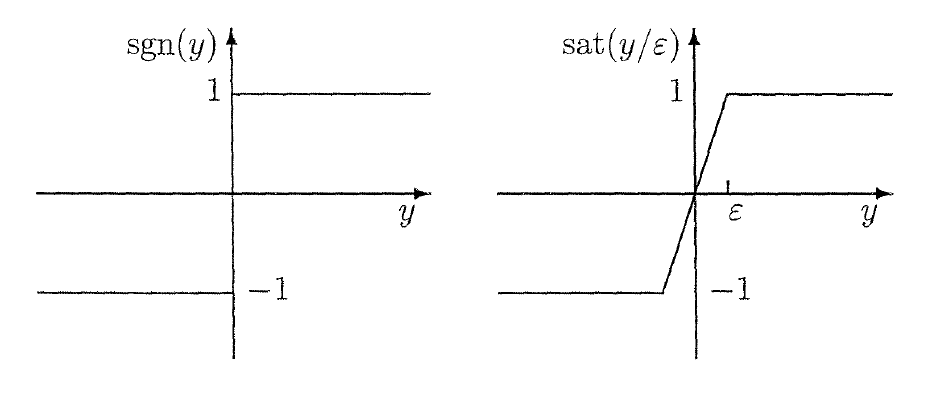
\includegraphics[width=0.6\textwidth]{saturation}
  \caption{Signum function (left) and the saturation function (right).}
  \label{fig:sign_sat}
\end{figure}
This strategy can, however, give rise to a fair amount of chattering in the system. To alleviate this we define a
constant, $\epsilon$. The constant $\epsilon$ is used to define a region close to the sliding surface where, when
within, the sign$()$ function is replaced with an approximation of a discontinous function - a saturation function.
\begin{equation}
  u = -\beta\left( \vect{x} \right) \up{sat}\left( \frac{s}{\epsilon} \right)
\end{equation}
Where:
\begin{equation}
  \up{sat}\left( \frac{s}{\epsilon} \right) =
  \begin{cases}
    \frac{s}{\epsilon} &\quad \text{if $\vert\frac{s}{\epsilon}\vert$ $\leq$ 1} \\[2mm]
    \up{sign}\left( \frac{s}{\epsilon} \right) &\quad \text{if $\vert \frac{s}{\epsilon}\vert$ $>$ 1}
  \end{cases}
\end{equation}

\begin{equation}
        u = -\left \vert \frac{a_1 x_2 + \hat{h}(x)}{\hat{g}(x)} \right\vert + v
\end{equation}
\begin{equation}
        \dot{s} = a_1\left(1 - \frac{c}{\hat{c}}\right) x_2 + \left(\frac{c}{\hat{c}} - 1\right)\hat{a} \sin x_1 + \left(\frac{c}{\hat{c}}\hat{b} - b\right) x_2 + cv + \xi(t) \doteq \delta(t) + cv
\end{equation}
\begin{equation}
        \left \vert \frac{\delta(t)}{g(x)} \right\vert \leq \varrho(x)
\end{equation}
\begin{equation}
        \left \vert \frac{\delta(t)}{g(x)} \right\vert = \left \vert \frac{\hat{a}c-\hat{a}\hat{c}}{c\hat{c}} \right \vert \vert \sin x_1 \vert + \left \vert \frac{a_1 - b}{c} + \frac{\hat{b} - a_1}{\hat{c}} \right \vert \vert x_2 \vert + \left\vert \frac{1}{c}\right\vert \left\vert \xi(t) \right\vert \leq \varrho(x)
\end{equation}
\begin{equation}
        u = -\beta(x)\up{sat}\left(\frac{s}{\epsilon}\right)
\end{equation}
where
\begin{equation}
        \beta(x) \geq \varrho(x) + \beta_0
\end{equation}


